%
% This is a borrowed LaTeX template file for lecture notes for CS267,
% Applications of Parallel Computing, UCBerkeley EECS Department.
% Now being used for CMU's 10725 Fall 2012 Optimization course
% taught by Geoff Gordon and Ryan Tibshirani.  When preparing 
% LaTeX notes for this class, please use this template.
%
% To familiarize yourself with this template, the body contains
% some examples of its use.  Look them over.  Then you can
% run LaTeX on this file.  After you have LaTeXed this file then
% you can look over the result either by printing it out with
% dvips or using xdvi. "pdflatex template.tex" should also work.
%

\documentclass[twoside]{article}
\setlength{\oddsidemargin}{0.25 in}
\setlength{\evensidemargin}{-0.25 in}
\setlength{\topmargin}{-0.6 in}
\setlength{\textwidth}{6.5 in}
\setlength{\textheight}{8.5 in}
\setlength{\headsep}{0.75 in}
\setlength{\parindent}{0 in}
\setlength{\parskip}{0.1 in}

%
% ADD PACKAGES here:
%

\usepackage{amsmath,amsfonts,graphicx}

%
% The following commands set up the lecnum (lecture number)
% counter and make various numbering schemes work relative
% to the lecture number.
%
\newcounter{lecnum}
\renewcommand{\thepage}{\thelecnum-\arabic{page}}
\renewcommand{\thesection}{\thelecnum.\arabic{section}}
\renewcommand{\theequation}{\thelecnum.\arabic{equation}}
\renewcommand{\thefigure}{\thelecnum.\arabic{figure}}
\renewcommand{\thetable}{\thelecnum.\arabic{table}}

%
% The following macro is used to generate the header.
%
\newcommand{\lecture}[4]{
   \pagestyle{myheadings}
   \thispagestyle{plain}
   \newpage
   \setcounter{lecnum}{#1}
   \setcounter{page}{1}
   \noindent
   \begin{center}
   \framebox{
      \vbox{\vspace{2mm}
    \hbox to 6.28in { {\bf ROB501 - Fundamentals \& Emerging Topics in Robotics - Digital Control Systems } }
       \vspace{4mm}
       \hbox to 6.28in { {\Large \hfill Lecture #1 \hfill} }
       \vspace{2mm}
       \hbox to 6.28in { {\it Lecturer: #2 \hfill } }
      \vspace{2mm}}
   }
   \end{center}
   \markboth{Lecture #1}{Lecture #1}

   \vspace*{4mm}
}
%
% Convention for citations is authors' initials followed by the year.
% For example, to cite a paper by Leighton and Maggs you would type
% \cite{LM89}, and to cite a paper by Strassen you would type \cite{S69}.
% (To avoid bibliography problems, for now we redefine the \cite command.)
% Also commands that create a suitable format for the reference list.
\renewcommand{\cite}[1]{[#1]}
\def\beginrefs{\begin{list}%
        {[\arabic{equation}]}{\usecounter{equation}
         \setlength{\leftmargin}{2.0truecm}\setlength{\labelsep}{0.4truecm}%
         \setlength{\labelwidth}{1.6truecm}}}
\def\endrefs{\end{list}}
\def\bibentry#1{\item[\hbox{[#1]}]}

%Use this command for a figure; it puts a figure in wherever you want it.
%usage: \fig{NUMBER}{SPACE-IN-INCHES}{CAPTION}
\newcommand{\fig}[3]{
			\vspace{#2}
			\begin{center}
			Figure \thelecnum.#1:~#3
			\end{center}
	}
% Use these for theorems, lemmas, proofs, etc.
\newtheorem{theorem}{Theorem}[lecnum]
\newtheorem{lemma}[theorem]{Lemma}
\newtheorem{proposition}[theorem]{Proposition}
\newtheorem{claim}[theorem]{Claim}
\newtheorem{corollary}[theorem]{Corollary}
\newtheorem{definition}[theorem]{Definition}
\newenvironment{proof}{{\bf Proof:}}{\hfill\rule{2mm}{2mm}}

% **** IF YOU WANT TO DEFINE ADDITIONAL MACROS FOR YOURSELF, PUT THEM HERE:

\begin{document}

% Lecture Details
\lecture{5}{Asst. Prof. M. Mert Ankarali}


\section{Steady-Sate (DC) Response Analysis}

Let's remember the final value theorem. Given a discrete time signal 
$x[k]$ and its z-transform $X(z)$,if $X(z)$ has no poles outside the
unit circle, then, final value theorem states that
%
\begin{align*}
\lim_{k\to \infty} x[k] &= \lim_{z \to 1} \left[ \left( 1 - z^{-1} \right)
  X(z) \right]
\\
x_{ss} &= \lim_{z \to 1} \left[ \frac{z-1}{z} X(z) \right]
\end{align*}

    \begin{center}
\begin{minipage}[h]{0.99\linewidth}
    \begin{center}
      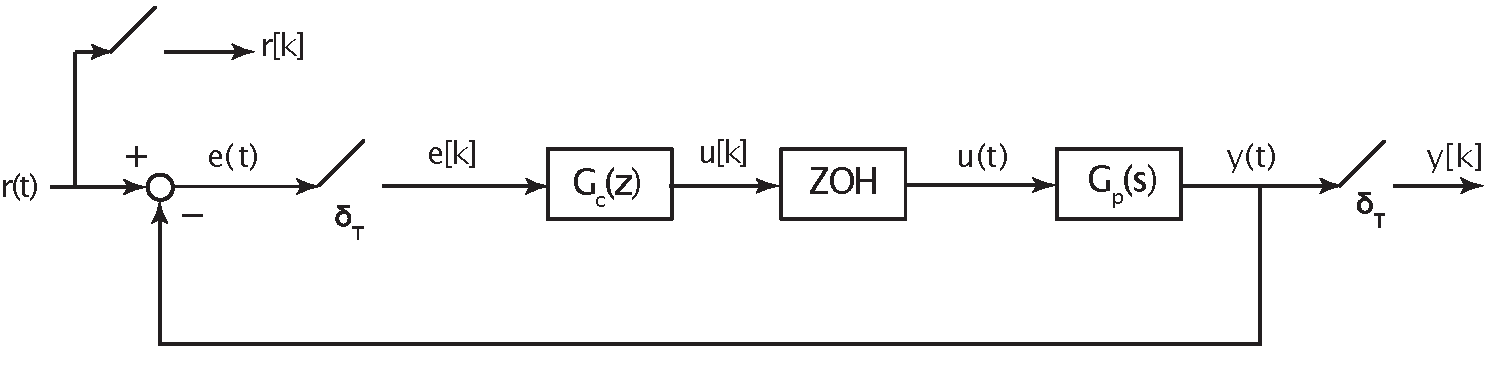
\includegraphics[width=\textwidth]{digitalblock}
    \end{center}
\end{minipage}
    \end{center}

Now let's find the pulse transfer function from the reference signal
$r[k]$ to the error signal $e[k]$, to further analyze the steady-state
error response. 
%
\begin{align*}
E(z) &= R(z) - E(z) \left( G_c(z) G(z) \right) , \quad \mathrm{where} \
  G(z) = \mathcal{Z} \lbrace G(s) \rbrace
\\
\frac{E(z)}{R(z)} &= \frac{1}{1 + G_c(z) G(z) }
\end{align*}
%
Note that $G_c(z) G(z)$ is the pulse transfer function from the error
signal $E(z)$ to the signal which is fed to the negative terminal of 
the main difference operator, i.e. $F(z)$. This transfer function is
called feed-forward or open-loop  pulse transfer function of the 
closed-loop digital control system. For this system, 
%
\begin{align*}
\frac{F(z)}{E(z)} = G_{OL} = G_c(z) G(z)
\end{align*}
%
Then $E(z)$ can be written as
%
\begin{align*}
E(z) = R(z) \frac{1}{1 + G_{OL} (z) }
\end{align*}
%
It is obvious that first requirement on m steady-state error
performance is that closed-loop system have to be stable.
Now let's analyze specific but fundamental input scenarios. 

\subsection*{Unit-Step Input}

We know that $r[k] = u[k]$ and $R(z) = \frac{1}{1 - z^-1}$ then 
we have
%
%
\begin{align*}
e_{ss} &= \lim_{z \to 1} \left[ \left(1 - z^{-1} \right) R(z) \frac{1}{1
         + G_{OL} (z) } \right]
\\
&= \lim_{z \to 1} \left[ \left(1 - z^{-1} \right) \frac{1}{1-z^{-1}} \frac{1}{1
         + G_{OL} (z) } \right]
\\
e_{ss} &= \frac{1}{1 + \lim_{z \to 1} G_{OL} (z) }
\end{align*}
%
If the DC gain of the system (also called static error constant) is
constant, i.e. $G_{OL}(1) = K_{DC}$ then the steady state error can be
computed as
%
\begin{align*}
e_{ss} &= \frac{1}{1 + K_{DC}}
\end{align*}
%
It is obvious that 
%
\begin{align*}
e_{ss} &\neq 0 \quad \mathrm{if} \quad |K_{DC}| < \infty
\\
e_{ss} &\to 0 \quad \mathrm{if} \quad K_{DC} \to \infty
\end{align*}
%
Based on these results, we can have the following conclusions
%
\begin{itemize}
\item If $G_{OL} (1) = K_{DC}$ , $0 < | K_{DC} | < \infty$, then $e_{ss} =
  1/(1 + K_{DC})$. These are \textbf{type 0} systems. We observe a
  bounded steady-state error and it is possible to reduce the by increasing the static gain
constant $K_P$. 
\item  If $G_{OL} (1) = \infty$, then $e_{ss} = 0$. These are
  \textbf{type \textit{positive}} systems. The steady-state error
  is perfectly zero for such systems.
\end{itemize}

Now let's generalize the \textit{type} of systems. An \textit{N type}
closed loop system has the following form of open-loop pulse transfer 
function
%
\begin{align*}
G_{OL}(z) &= \frac{1}{(z-1)^N} G_{DC}(z) \\
| G_{DC}(1) | &= K_{DC} \quad \mathrm{where} \ 0 < | K_{DC} | < \infty
\end{align*}
% 
It is easy to see that for unit-step response
%
\begin{itemize}
\item Type $N = 0$: $e_{ss} =  1/(1 + K_{DC})$
\item Type $N > 0$: $e_{ss} = 0$
\end{itemize}

\newpage

\subsection*{Unit-Ramp Input}
%
We know that $r[k] = k u[k]$ and $R(z) = \frac{z^{-1}}{(1 - z^{-1})^2}$ then
we have

\begin{align*}
e_{ss} &= \lim_{z \to 1} \left[ \left(1 - z^{-1} \right) R(z) \frac{1}{1
         + G_{OL} (z) } \right]
\\
&= \lim_{z \to 1} \left[ \left(1 - z^{-1} \right) 
  \frac{z^{-1}}{(1 - z^{-1})^2} \frac{1}{1 +\frac{1}{(z-1)^N} G_{DC}(z) } \right]
\\
&= \lim_{z \to 1} \left[ \frac{1}{z - 1} \frac{1}{1 +\frac{1}{(z-1)^N}
  G_{DC}(z) } \right]
\\
&= \lim_{z \to 1} \left[ \frac{1}{(z-1) +\frac{1}{(z-1)^{N-1}}
  G_{DC}(z) } \right]
\\
e_{ss} &=  \frac{1}{ \lim_{z \to 1} \left[ \frac{1}{(z-1)^{N-1}}
  G_{DC}(z) \right] }
\end{align*}
%
Based on this result we can have the following steady-state
error conditions for the unit-ramp input based on the type 
condition of the system
%
\begin{itemize}
\item Type $N < 1$: $e_{ss} \to  \infty$
\item Type $N = 1$: $e_{ss} = \frac{1}{K_{DC}}$
\item Type $N > 1$: $e_{ss} = 0$
\end{itemize}

\paragraph{Example 1:} $G_{OL}(z) = K \frac{z}{z-0.5}$. Compute the steady-state error to unit-step, and unit-ramp inputs.
%
\begin{align*}
G_{OL}(z) &= \frac{K z}{z-0.5} 
\\
G_{DC}(1) &= 2 K \quad, \mathrm{Type} \ 0 
\end{align*}
%
Then the steady-state errors are computed as
%
\begin{itemize}
\item Unit-step: $e_{ss} = \frac{1}{1 + 2 K}$
\item Unit-ramp: $e_{ss} = \infty$
\end{itemize}

\paragraph{Example 2:} $G_{OL}(z) =
K \frac{z^2}{(z-1)(z-0.5)}$. Compute the steady-state erro to unit-step, unit-ramp, a
and unit-quadratic inputs.

%
\begin{align*}
G_{OL}(z) &= \frac{K z^2}{(z-1) (z-0.5)} = \frac{1}{z-1} \frac{K
            z^2}{z - 0.5}
\\
G_{DC}(1) &= 2 K \quad, \mathrm{Type} \ 1 
\end{align*}
%
Then the steady-state errors are computed as
%
\begin{itemize}
\item Unit-step: $e_{ss} = 0$
\item Unit-ramp: $e_{ss} = \frac{1}{2 K}$
\end{itemize}


% **** This ENDS THE EXAMPLES. DON'T DELETE THE FOLLOWING LINE:
\end{document}
